\subsubsection{Analisis Skenario Layanan Kesehatan Kolaboratif}
\label{subsubsec:analisis-skenario-layanan-klinis}
Kebutuhan akan kontrol akses granular dan delegasi berantai menjadi lebih jelas ketika arsitektur DecMed ditempatkan pada skenario layanan kesehatan yang nyata. Dalam alur pelayanan rumah sakit, pasien tidak hanya berinteraksi dengan satu pihak, tetapi dengan beberapa aktor yang memiliki kebutuhan akses berbeda pada tahap yang berbeda pula. Oleh karena itu, subbab ini memodelkan satu skenario layanan kesehatan kolaboratif untuk menunjukkan secara konkret mengapa mekanisme akses pada DecMed saat ini belum memadai.

Skenario yang dianalisis adalah pelayanan pasien rawat jalan yang melibatkan petugas administrasi, dokter penanggung jawab pasien, dan unit laboratorium. Alur tersebut dipilih karena mewakili pola kolaborasi yang umum terjadi di fasilitas pelayanan kesehatan, sekaligus cukup untuk memperlihatkan kebutuhan akses baca, tulis, dan delegasi terbatas. Kebutuhan delegasi ini berkaitan dengan kebutuhan fungsional DecMed pada Lampiran \ref{lampiran:kebutuhan-fungsional-decmed}, khususnya ID F06 dan F07.

\begin{enumerate}[leftmargin=*]
	\item \textbf{Tahap pendaftaran pasien.} Saat pasien datang ke rumah sakit, petugas administrasi membutuhkan akses terhadap data identitas, nomor rekam medis, informasi penjamin, dan data pendaftaran kunjungan. Pada tahap ini, petugas administrasi tidak memerlukan akses terhadap riwayat diagnosis, hasil laboratorium sebelumnya, atau catatan terapi pasien.
	\item \textbf{Tahap pemeriksaan awal oleh dokter.} Setelah proses pendaftaran selesai, dokter penanggung jawab pasien memerlukan hak baca terhadap riwayat klinis yang relevan, seperti keluhan sebelumnya, diagnosis terdahulu, alergi, obat yang sedang dikonsumsi, dan hasil pemeriksaan penunjang yang masih berkaitan. Selain itu, dokter juga membutuhkan hak tulis untuk menambahkan anamnesis, hasil pemeriksaan fisik, diagnosis kerja, dan rencana tindak lanjut.
	\item \textbf{Tahap rujukan internal ke laboratorium.} Apabila dokter membutuhkan pemeriksaan laboratorium, maka dokter perlu meneruskan sebagian hak akses kepada petugas laboratorium. Dalam tahap ini, petugas laboratorium hanya membutuhkan akses terhadap identitas minimum pasien yang diperlukan untuk verifikasi sampel, permintaan pemeriksaan, serta hak tulis untuk mengunggah hasil pemeriksaan. Petugas laboratorium tidak memerlukan akses penuh terhadap seluruh riwayat klinis pasien.
	\item \textbf{Tahap tindak lanjut hasil pemeriksaan.} Setelah hasil laboratorium tersedia, dokter kembali menggunakan data tersebut sebagai bahan pengambilan keputusan klinis. Alur ini menunjukkan bahwa akses terhadap RME bersifat bertahap, berpindah antarpihak, dan berubah sesuai konteks layanan.
\end{enumerate}

Berdasarkan skenario tersebut, kebutuhan akses setiap aktor dapat diringkas pada Tabel \ref{tab:skenario-layanan-kolaboratif}.

\begin{table}[!ht]
	\centering
	\caption{Pemetaan Aktor dan Kebutuhan Akses pada Skenario Layanan Kesehatan Kolaboratif}
	\label{tab:skenario-layanan-kolaboratif}
	\small
	\begin{tabular}{|p{0.2\textwidth}|p{0.23\textwidth}|p{0.45\textwidth}|}
		\hline
		\textbf{Aktor}                 & \textbf{Jenis Akses}              & \textbf{Cakupan Data yang Dibutuhkan}                                                       \\ \hline
		Petugas administrasi           & Baca dan tulis data administratif & Data administratif pasien.                                                                  \\ \hline
		Dokter penanggung jawab pasien & Baca dan tulis data klinis        & Riwayat klinis yang relevan, hasil pemeriksaan, diagnosis, dan rencana terapi.              \\ \hline
		Petugas laboratorium           & Baca terbatas dan tulis terbatas  & Identitas minimum pasien, detail permintaan pemeriksaan, serta unggahan hasil laboratorium. \\ \hline
	\end{tabular}
\end{table}
Alur pemberian akses medis pada DecMed sesuai dengan implementasi saat ini dapat dilihat pada Gambar \ref{fig:patient-create-access-medical-personnel}. Pada alur tersebut, pasien harus memilih satu tenaga medis lalu menerbitkan token akses untuk tenaga medis tersebut. Apabila akses perlu diberikan kepada lebih dari satu tenaga medis, proses yang sama perlu diulang dari awal untuk masing-masing penerima akses.

\begin{figure}[!ht]
	\centering
	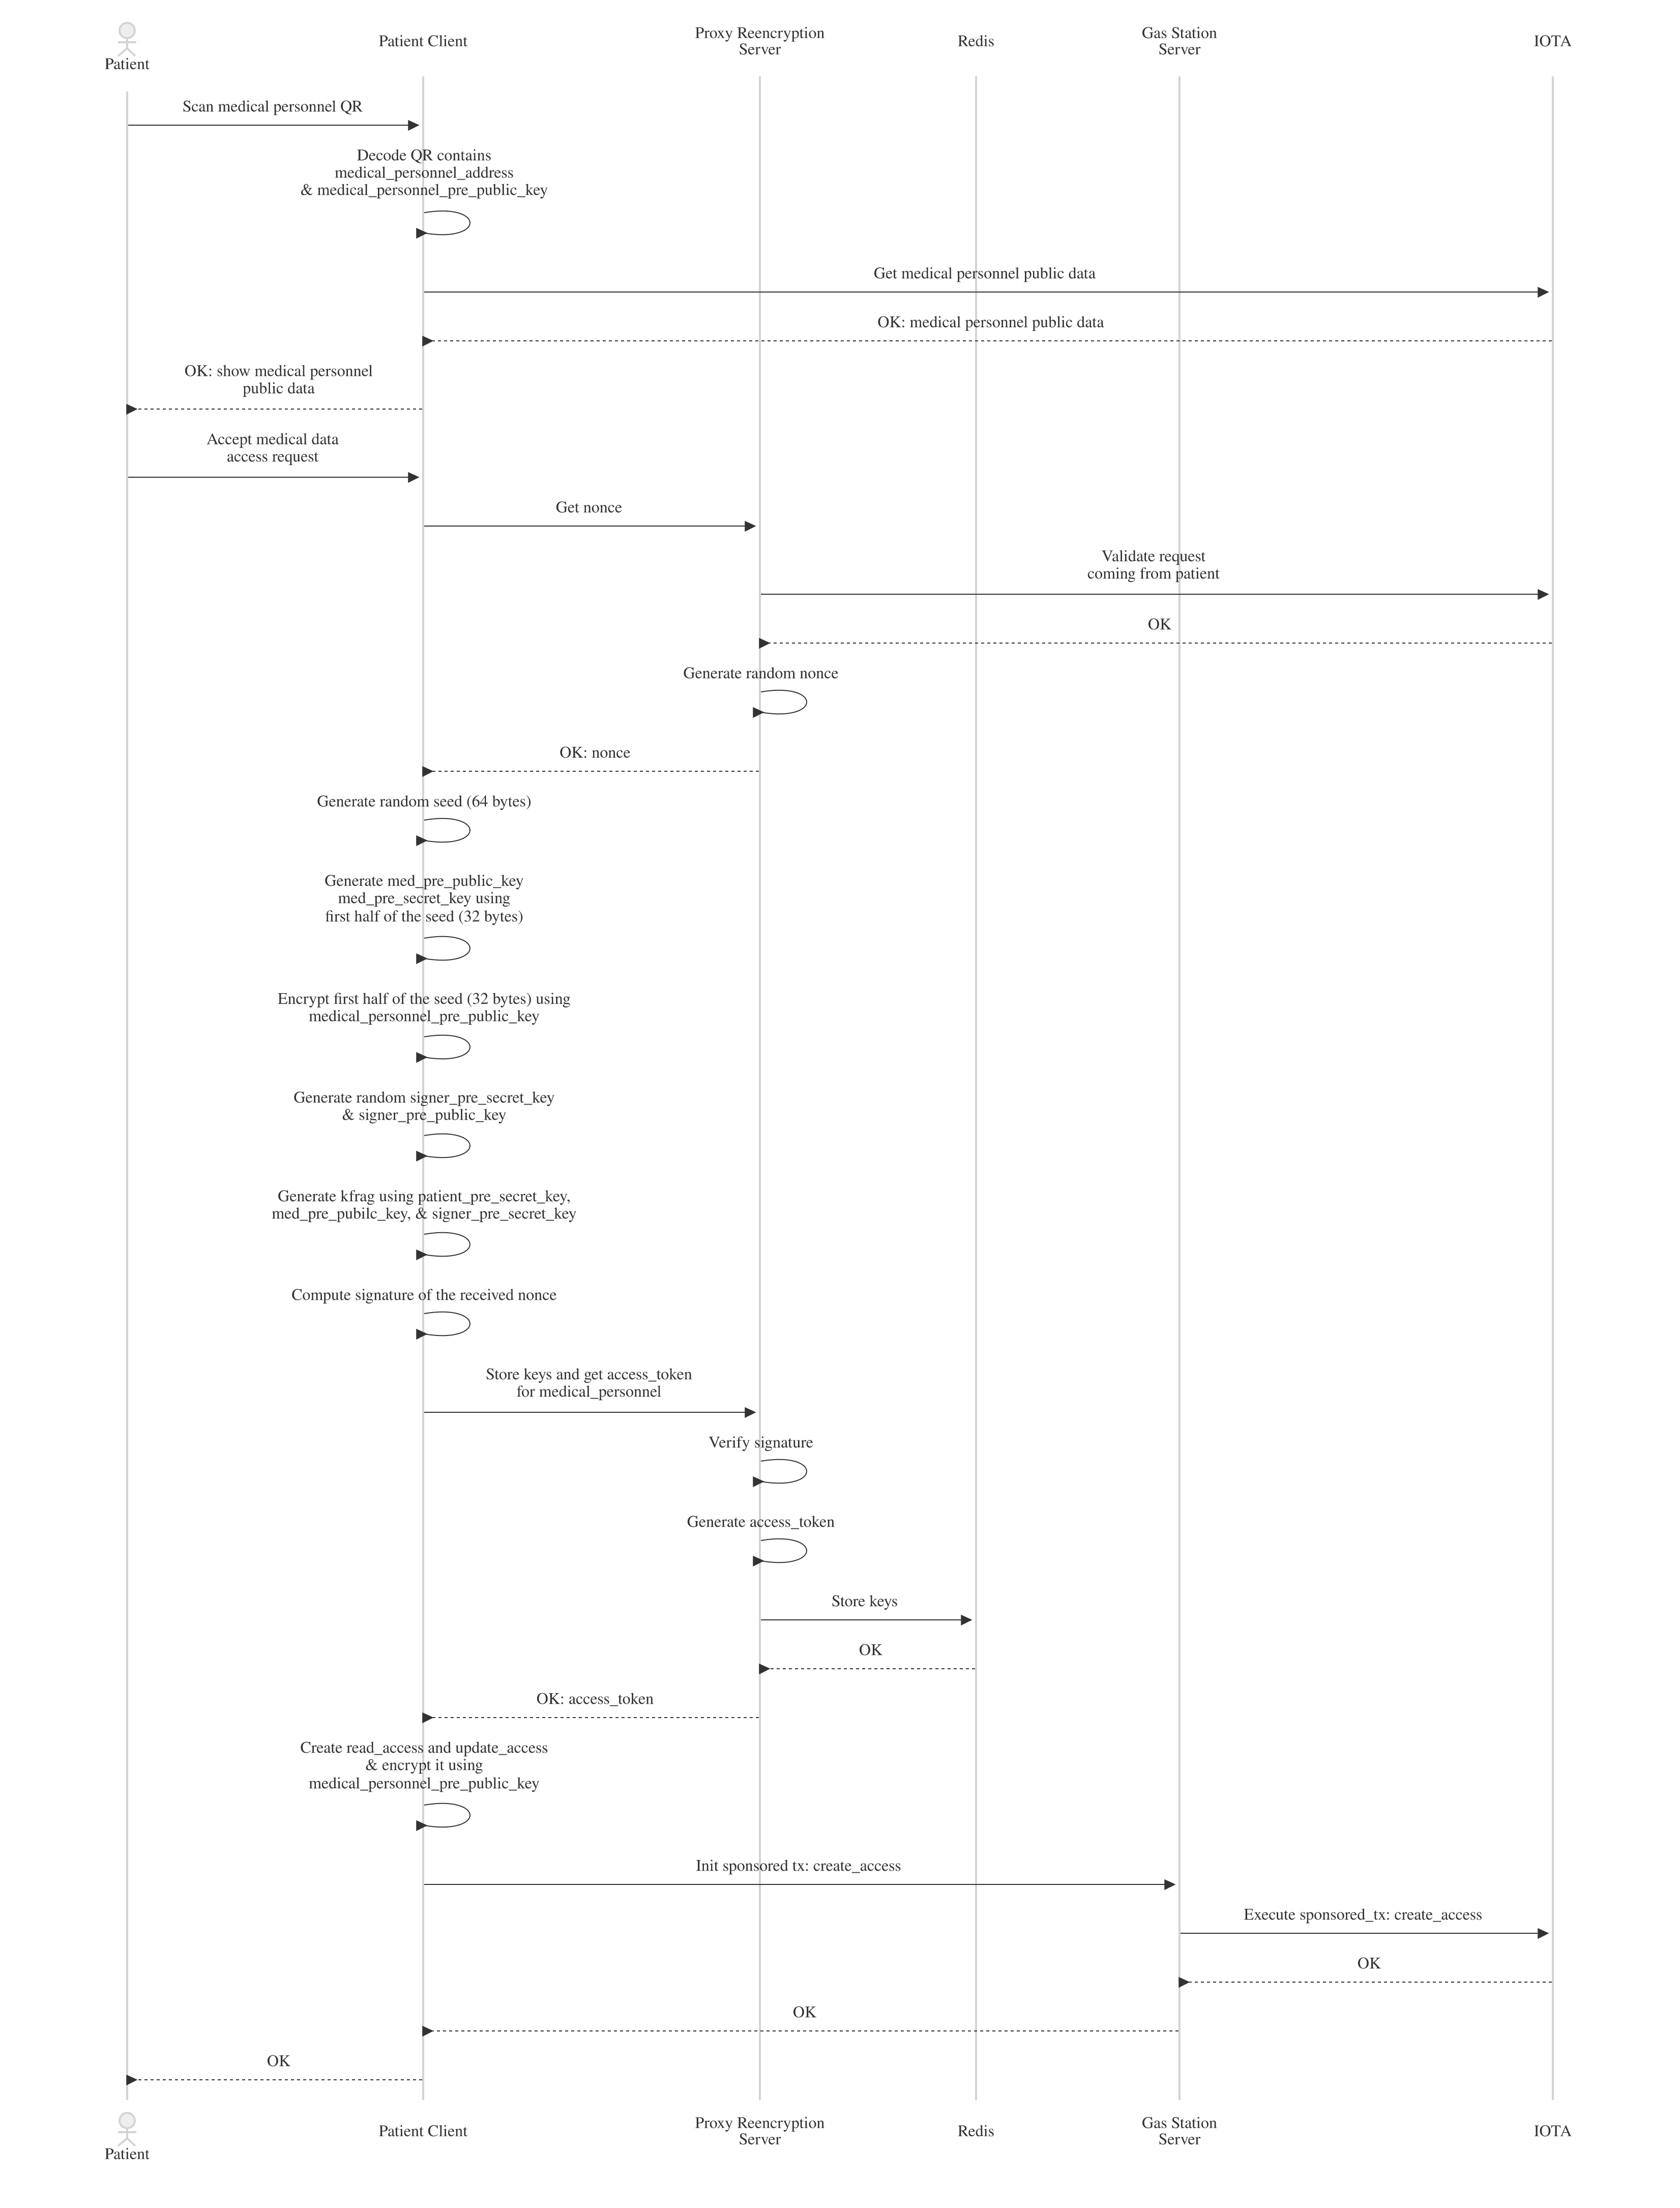
\includegraphics[width=1\textwidth]{resources/chapter-3/analisis/patient_create_access_for_medical_personnel_svg.png}
	\caption{\textit{Sequence diagram} alur pemberian akses medis dari pasien kepada tenaga medis \autocite{sadewa2025decmed}}
	\label{fig:patient-create-access-medical-personnel}
\end{figure}

Dalam skenario tersebut, keterbatasan DecMed tampak secara operasional. Model token kapabilitas yang statis menyulitkan proses pembatasan akses secara bertahap sesuai perpindahan peran di lapangan. Selain itu, pemberian akses hanya dapat dilakukan secara individual dari pasien kepada satu tenaga medis pada satu waktu, sehingga proses otorisasi menjadi tidak efektif ketika layanan melibatkan beberapa tenaga medis sekaligus. Dokter tidak cukup hanya ``membuka'' atau ``menutup'' akses, tetapi perlu mendelegasikan sebagian haknya saja, misalnya akses terhadap permintaan pemeriksaan dan hak tulis hasil laboratorium tanpa ikut membuka seluruh riwayat klinis pasien. Jika data klinis masih tersimpan dalam unit \textit{off-chain} yang terlalu besar, maka pemberian akses kepada unit laboratorium juga berisiko membuka data yang tidak relevan.

Selain itu, apabila setiap delegasi baru tetap mensyaratkan penerbitan ulang token oleh pasien, maka alur kerja klinis akan terhambat karena pasien harus terus dilibatkan untuk kebutuhan otorisasi yang bersifat teknis. Kondisi ini tidak selaras dengan praktik pelayanan yang kolaboratif dan dinamis. Dokter penanggung jawab pasien dapat perlu mendelegasikan sebagian hak akses kepada residen, perawat, atau unit laboratorium tanpa menunggu kehadiran pasien. Pada fasilitas seperti rumah sakit, keterlibatan ulang pasien untuk setiap tenaga medis yang menangani pasien juga berpotensi mengganggu alur pelayanan. Dengan demikian, skenario layanan kesehatan kolaboratif ini memperlihatkan bahwa tiga persoalan penelitian saling berkaitan: sistem memerlukan kontrol akses yang granular agar setiap aktor hanya memperoleh data yang relevan, segmentasi data \textit{off-chain} agar pembatasan akses dapat ditegakkan secara teknis, dan delegasi berantai dengan atenuasi luring agar perpindahan hak akses dapat berlangsung efisien tanpa intervensi ulang dari pasien.
